\begin{figure}
    \centering
\begin{knitrout}
\definecolor{shadecolor}{rgb}{0.969, 0.969, 0.969}\color{fgcolor}
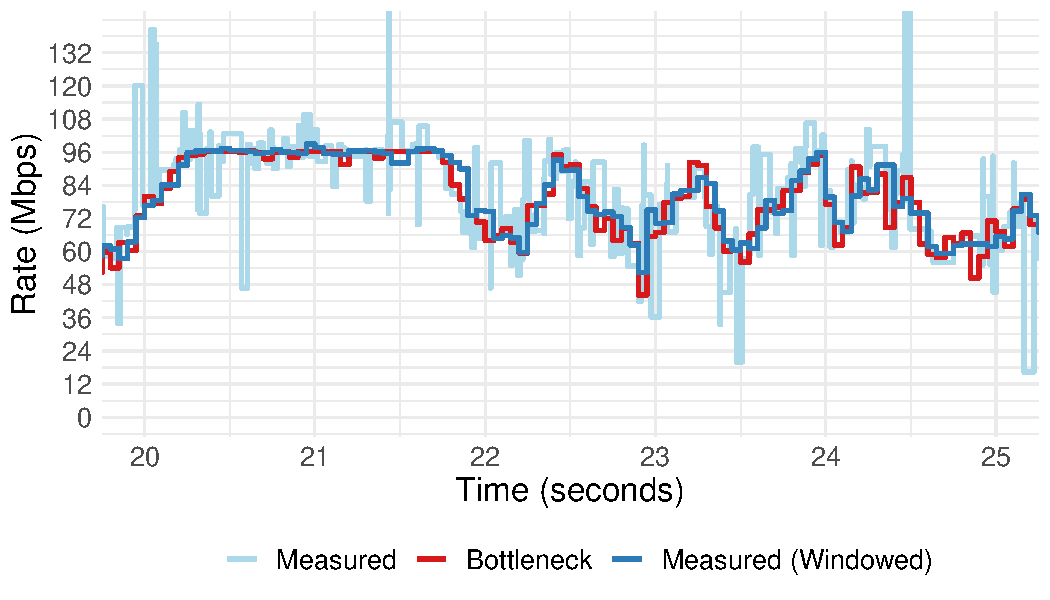
\includegraphics[width=\maxwidth]{figure/micro:time-1} 

\end{knitrout}
    \caption{\name's estimate of the receive rate compared to the actual rate leaving the bottleneck over a five second trace. 
    \name's raw estimate of the rate hovers around the true value, but is noisy. Averaging over a window of previous epochs
    yields a much smoother estimate that closely matches the true value.}
    \label{fig:micro:time}
\end{figure}
